\chapter{Digital Submission of Reports}
\label{app:submission} % Always give a unique label


Each project you do this semester will involve several pieces: Code, Images, and \LaTeX\ code. 
In order to make it easier for me to give timely feedback and to facilitate my record keeping, I am asking everyone
to follow a very specific format for both the naming and organization of submitted projects. I will now describe this structure in detail (you'll see that the format is really quite simple); however, keep in mind that
submitted projects that do not follow this structure will be returned and will need to be re-submitted
and will result in a 10\% penalty. 

I will be asking each of you to submit your reports electronically as a single compressed file (in Linux or Mac OS, just right click on a folder to bring up a dialog option to compress the folder.) 

\section{Folder Structure}\label{sec:Folders}
The folder structure is really quite simple, and Figure~\ref{fig:FolderScheme} shows the general layout; there is a single top level folder, which contains four sub-folders which delineate the major pieces of each assignment. Of these four sub-folders, only the LaTeX folder has one more sub-folder. 
\begin{figure}[htb]
  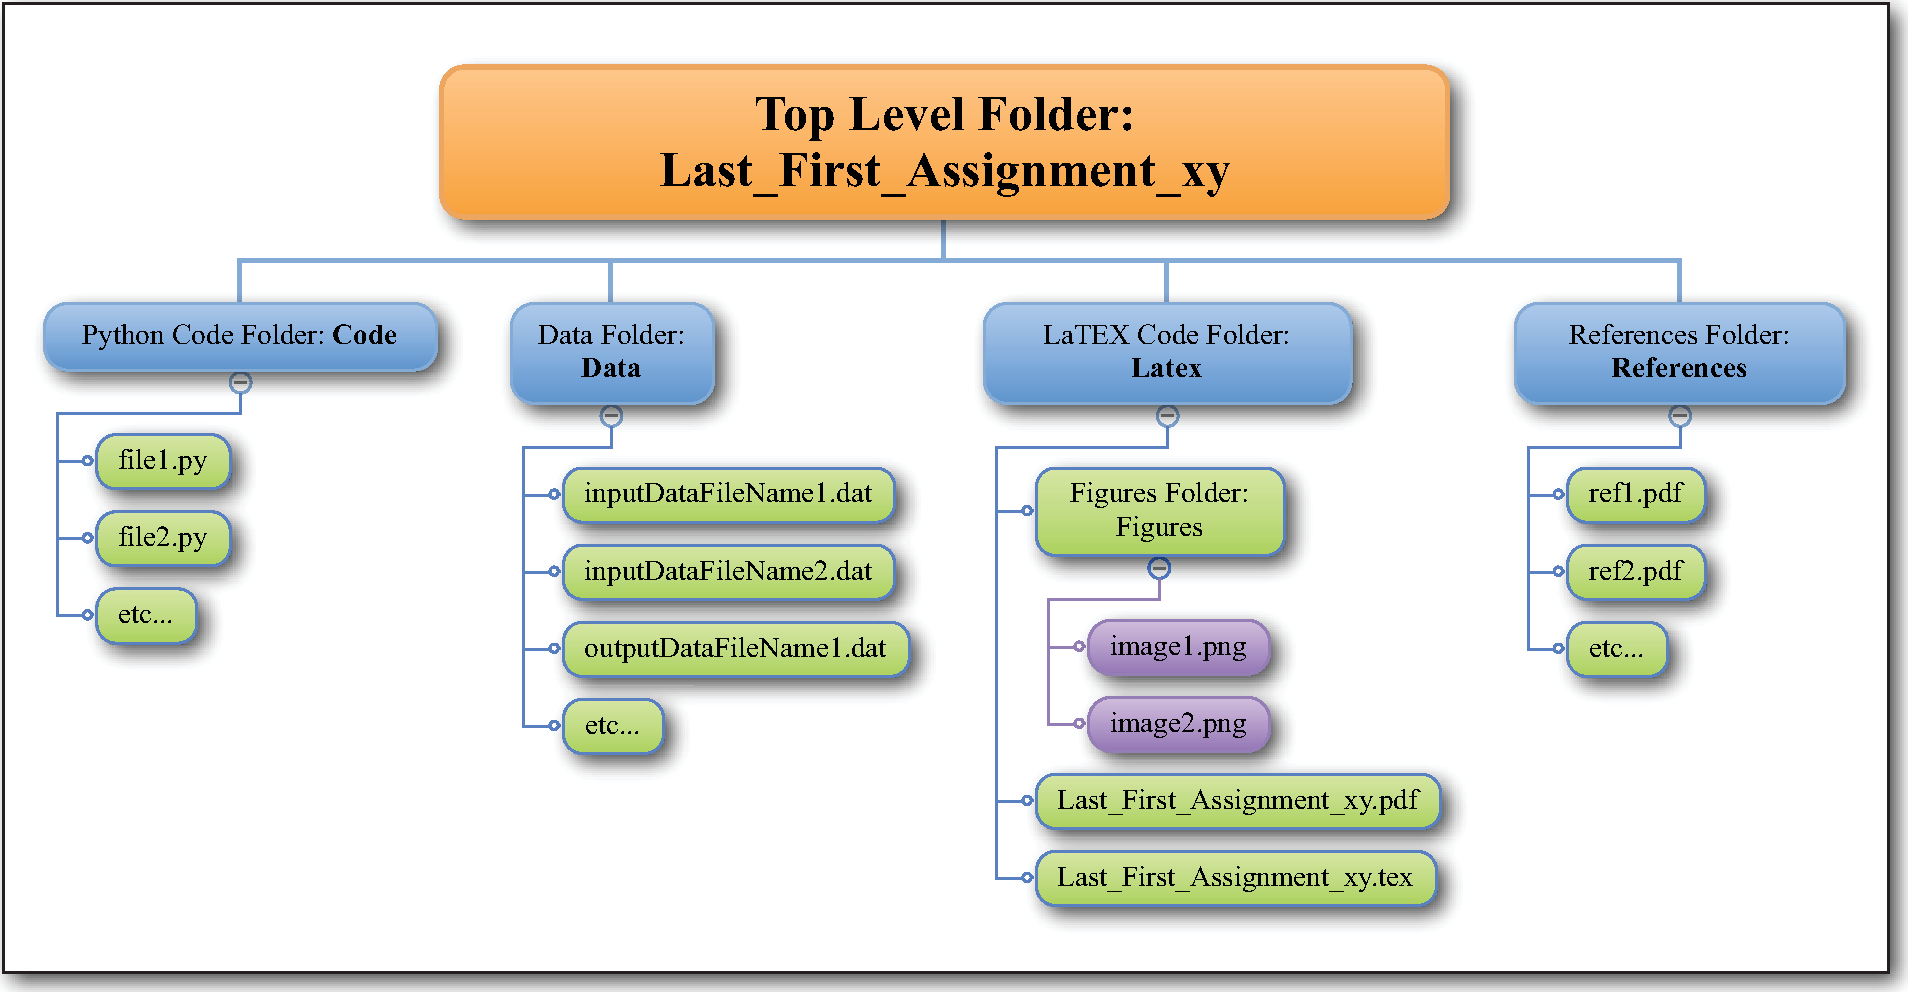
\includegraphics[width=\linewidth]{Figures/digitalSubmission/FolderScheme.pdf}%
  \caption{You will submit a top level folder with four immediate sub-folders.
  The \LaTeX\ folder will also have one sub-folder containing all the figures generated by either Python code you wrote, or by a drawing program such as \emph{Inkscape}.}
  \label{fig:FolderScheme}
\end{figure}

After you understand the general scheme for structuring your assignment submission, you can see a specific example in Figure~\ref{fig:exampleSubmission}. Please email your assignment to me at \verb!pauln@maine.edu!, with subject line: \verb!PHY261 Assignment 01! (for example).

\begin{figure}[]
	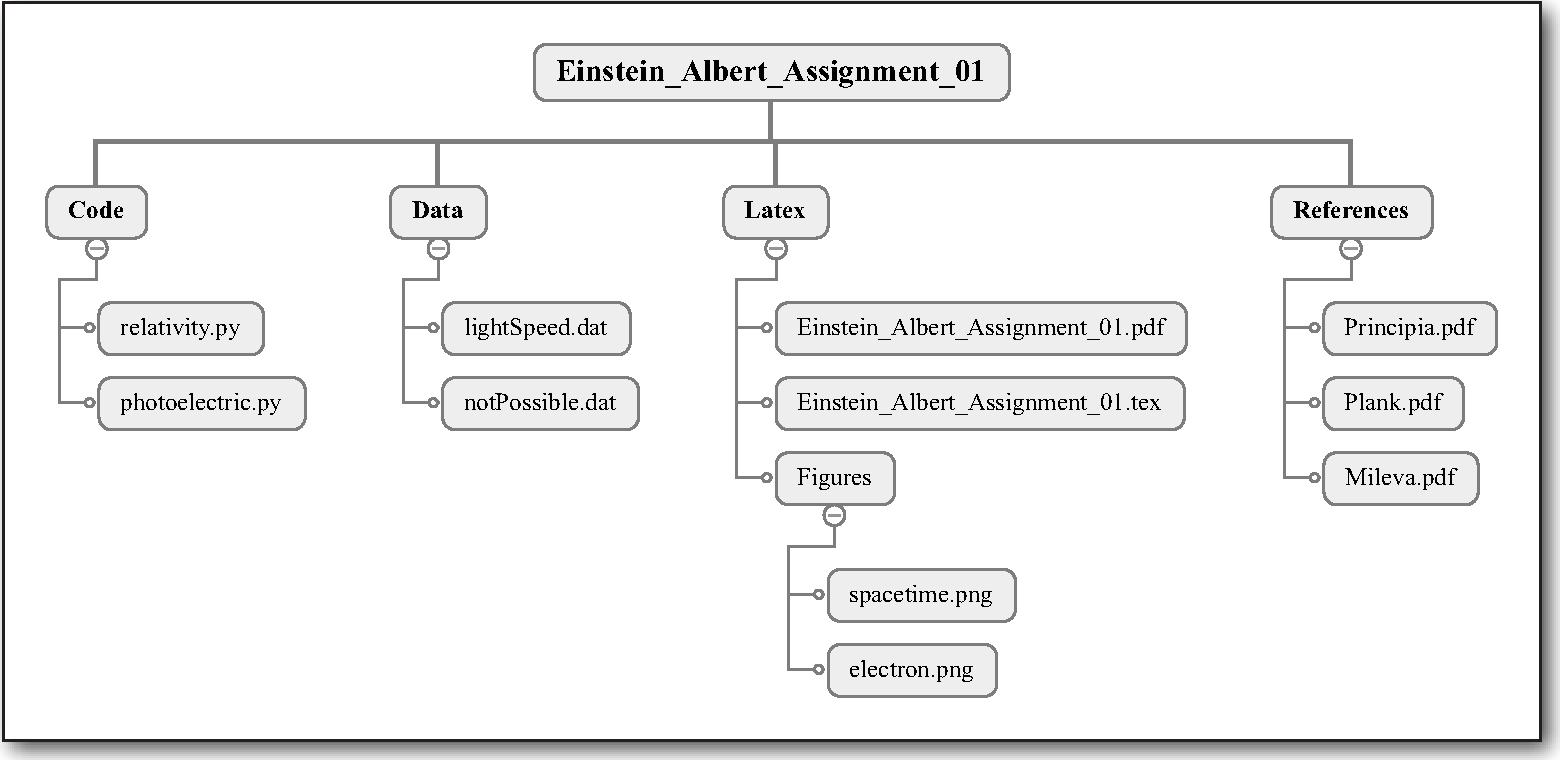
\includegraphics[width=\linewidth]{Figures/digitalSubmission/Example.pdf}
	\caption{Here is a specific example of an assignment submission by a former student of
	physics. Note that said student would send me a compressed version of the top level folder.}\label{fig:exampleSubmission}
\end{figure}
